% This LaTeX document needs to be compiled with XeLaTeX.
\documentclass[
  10
]{article}
\usepackage[margin=2cm,includehead=true,includefoot=true,centering,]{geometry}
\usepackage{xcolor}
\usepackage{ucharclasses}
\usepackage{hyperref}
\usepackage{amsmath,amssymb}
\usepackage{amsfonts}
\usepackage[version=4]{mhchem}
\usepackage{stmaryrd}
\usepackage{bbold}
\usepackage{polyglossia}
\usepackage{fontspec}
\usepackage{ctex}
\usepackage[export]{adjustbox}
\usepackage{tabularx}
\usepackage{booktabs}

\usepackage{setspace}
\setstretch{1.2}

\makeatletter
\@ifundefined{KOMAClassName}{% if non-KOMA class
  \IfFileExists{parskip.sty}{%
    \usepackage{parskip}
  }{% else
    \setlength{\parindent}{0pt}
    \setlength{\parskip}{6pt plus 2pt minus 1pt}}
}{% if KOMA class
  \KOMAoptions{parskip=half}}
\makeatother
\usepackage{longtable,booktabs,array}
\newcounter{none} % for unnumbered tables
\usepackage{calc} % for calculating minipage widths
% Correct order of tables after \paragraph or \subparagraph
\usepackage{etoolbox}
\makeatletter
\patchcmd\longtable{\par}{\if@noskipsec\mbox{}\fi\par}{}{}
\makeatother
% Allow footnotes in longtable head/foot
\IfFileExists{footnotehyper.sty}{\usepackage{footnotehyper}}{\usepackage{footnote}}
\makesavenoteenv{longtable}
\usepackage{graphicx}
\makeatletter
\newsavebox\pandoc@box
\newcommand*\pandocbounded[1]{% scales image to fit in text height/width
  \sbox\pandoc@box{#1}%
  \Gscale@div\@tempa{\textheight}{\dimexpr\ht\pandoc@box+\dp\pandoc@box\relax}%
  \Gscale@div\@tempb{\linewidth}{\wd\pandoc@box}%
  \ifdim\@tempb\p@<\@tempa\p@\let\@tempa\@tempb\fi% select the smaller of both
  \ifdim\@tempa\p@<\p@\scalebox{\@tempa}{\usebox\pandoc@box}%
  \else\usebox{\pandoc@box}%
  \fi%
}
% Set default figure placement to htbp
\def\fps@figure{htbp}
\makeatother
\setlength{\emergencystretch}{3em} % prevent overfull lines
\providecommand{\tightlist}{%
  \setlength{\itemsep}{0pt}\setlength{\parskip}{0pt}}


\hypersetup{colorlinks=true, linkcolor=blue, filecolor=magenta, urlcolor=cyan,}
\urlstyle{same}

\usepackage{colortbl}
\definecolor{table-row-color}{HTML}{999999}
\definecolor{table-rule-color}{HTML}{999999}
%\arrayrulecolor{black!40}
\arrayrulecolor{table-rule-color}     % color of \toprule, \midrule, \bottomrule
\setlength{\aboverulesep}{0pt}
\setlength{\belowrulesep}{0pt}


\setotherlanguages{english}
\IfFontExistsTF{Source Han Serif CN}
{\newfontfamily\chinesefont{Source Han Serif CN}}
{\IfFontExistsTF{Noto Serif CJK SC}
  {\newfontfamily\chinesefont{Noto Serif CJK SC}}
  {\IfFontExistsTF{SimSun}
    {\newfontfamily\chinesefont{SimSun}}
    {\IfFontExistsTF{FangSong}
      {\newfontfamily\chinesefont{FangSong}}
      {\newfontfamily\chinesefont{Arial Unicode MS}}
}}}
\IfFontExistsTF{Times New Roman}
{\newfontfamily\englishfont{Times New Roman}}
{\IfFontExistsTF{Liberation Serif}
  {\newfontfamily\englishfont{Liberation Serif}}
  {\IfFontExistsTF{DejaVu Serif}
    {\newfontfamily\englishfont{DejaVu Serif}}
    {\newfontfamily\englishfont{Arial}}
}}


\author{}
\date{}

\begin{document}


\section{Chebyshev polynomial filtered subspace iteration in the
discontinuous Galerkin method for large-scale electronic structure
calculations}\label{chebyshev-polynomial-filtered-subspace-iteration-in-the-discontinuous-galerkin-method-for-large-scale-electronic-structure-calculations}

Amartya S. Banerjee, Lin Lin, Wei Hu, Chao Yang, and John E. Pask

Citation: The Journal of Chemical Physics 145, 154101 (2016); doi:
10.1063/1.4964861

View online: http://dx.doi.org/10.1063/1.4964861

View Table of Contents:
http://scitation.aip.org/content/aip/journal/jcp/145/15?ver=pdfcov

Published by the AIP Publishing

\section{Articles you may be interested
in}\label{articles-you-may-be-interested-in}

DGDFT: A massively parallel method for large scale density functional
theory calculations

J. Chem. Phys. 143, 124110 (2015); 10.1063/1.4931732

Preconditioned iterative minimization for linear-scaling electronic
structure calculations

J. Chem. Phys. 119, 8842 (2003); 10.1063/1.1613633

Density matrix search using direct inversion in the iterative subspace
as a linear scaling alternative to diagonalization in electronic
structure calculations

J. Chem. Phys. 119, 7651 (2003); 10.1063/1.1607961

Vibrational eigenstates of NO 2 by a Chebyshev-MINRES spectral filtering
procedure

J. Chem. Phys. 117, 8314 (2002); 10.1063/1.1512651

Comparison of conjugate gradient density matrix search and Chebyshev
expansion methods for avoiding diagonalization in large-scale electronic
structure calculations

J. Chem. Phys. 109, 3308 (1998); 10.1063/1.476927

\pandocbounded{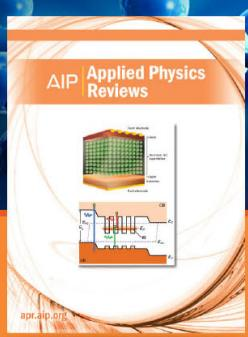
\includegraphics[keepaspectratio,alt={image}]{images/a1f802d2a21b67aa7c83d47b1f3c5240e0d28378e2b0e73567611ced92d22ce7.jpg}}

\section{NEW Special Topic Sections}\label{new-special-topic-sections}

Lithium Niobate Properties and Applications:

Reviews of Emerging Trends

\pandocbounded{
\includegraphics[keepaspectratio,alt={image}]{images/467a5a4eee6b2e731bb314f792276edd74aaf84d8692f1ee165dfaf480b94686.jpg}}

Reviews

\section{Chebyshev polynomial filtered subspace iteration in the
discontinuous Galerkin method for large-scale electronic structure
calculations}\label{chebyshev-polynomial-filtered-subspace-iteration-in-the-discontinuous-galerkin-method-for-large-scale-electronic-structure-calculations-1}

Amartya S. Banerjee,1,a) Lin Lin,1,2,b) Wei Hu,1,c) Chao Yang,1,d) and
John E. Pask3,e)

1Computational Research Division, Lawrence Berkeley National Laboratory,
Berkeley, California 94720, USA

2Department of Mathematics, University of California, Berkeley,
California 94720, USA

3Physics Division, Lawrence Livermore National Laboratory, Livermore,
California 94550, USA

(Received 10 June 2016; accepted 3 October 2016; published online 17
October 2016)

The Discontinuous Galerkin (DG) electronic structure method employs an
adaptive local basis (ALB) set to solve the Kohn-Sham equations of
density functional theory in a discontinuous Galerkin framework. The
adaptive local basis is generated on-the-fly to capture the local
material physics and can systematically attain chemical accuracy with
only a few tens of degrees of freedom per atom. A central issue for
large-scale calculations, however, is the computation of the electron
density (and subsequently, ground state properties) from the discretized
Hamiltonian in an efficient and scalable manner. We show in this work
how Chebyshev polynomial filtered subspace iteration (CheFSI) can be
used to address this issue and push the envelope in large-scale
materials' simulations in a discontinuous Galerkin framework. We
describe how the subspace filtering steps can be performed in an
efficient and scalable manner using a two-dimensional parallelization
scheme, thanks to the orthogonality of the DG basis set and block-sparse
structure of the DG Hamiltonian matrix. The on-the-fly nature of the ALB
functions requires additional care in carrying out the subspace
iterations. We demonstrate the parallel scalability of the DG-CheFSI
approach in calculations of large-scale twodimensional graphene sheets
and bulk three-dimensional lithium-ion electrolyte systems. Employing 55
296 computational cores, the time per self-consistent field iteration
for a sample of the bulk 3D electrolyte containing 8586 atoms is 90 s,
and the time for a graphene sheet containing 11 520 atoms is 75 s.
Published by AIP Publishing. {[}http://dx.doi.org/10.1063/1.4964861{]}

\section{I. INTRODUCTION}\label{i.-introduction}

Kohn-Sham Density functional theory (KS-DFT)1,2 is the most widely used
methodology for electronic structure calculations of condensed matter
and nano-material systems. KS-DFT requires the solution of a nonlinear
eigenvalue problem, and this is usually achieved by means of
selfconsistent field (SCF) iterations in conjunction with convergence
acceleration schemes.3,4 The most computationally intensive part of
conventional KS-DFT calculations is the solution of the linear
eigenvalue problem associated with diagonalization of the Kohn-Sham
Hamiltonian on every SCF step. The results of this eigenvalue problem
are used to update the electron density , from which the various ρterms
of the Kohn-Sham Hamiltonian are computed. As the SCF iterations
progress, the solution to the linear eigenvalue problem on successive
SCF steps forms increasingly better approximations to the actual
Kohn-Sham eigenstates.

The computational complexity (or algorithmic complexity) of the solution
of the linear eigenvalue problem, with respect to the number of
electronic states in the system, is dependent on the algorithm used for
solution of the eigenvalue problem --- in particular, it depends on
whether direct or iterative methods of solution are used. The prefactor
in such algorithmic complexity estimates strongly influences the
simulation wall times in practical computations. The ability to tackle
large-scale complex materials science problems, therefore, is closely
related to how small the prefactor can be made in real computations,
regardless of which diagonalization algorithm is used.

The prefactor is not only influenced by the choice of algorithm but also
by the discretization scheme. Specifically, it depends on the number of
basis functions per atom required to obtain accurate and reliable
results. The widely used planewave method3,5,6 allows high fidelity
calculations to be carried out since systematic convergence with respect
to the number of basis functions per atom can be obtained. However, this
method requires a large number of basis functions per atom --- often
thousands or more planewaves per atom need to be employed. Similar
observations hold true for methods based on finite elements,7--10 finite
differences,11--14 and other planewave-like spectral basis
functions.15,16 On the other hand, methods based on atom centered basis
functions17--20 typically require fewer basis functions per atom (often,
as few as 10--80). However, it can be nontrivial to improve the quality
of solutions obtained via such methods, as a result of which the success
of a practical calculation can depend on the experience of the
practitioner.

In a series of recent contribution s,21--24 a new methodology for
discretizing the Kohn-Sham equations using so-called adaptive local
basis (ALB) functions has been presented. This approach involves
partitioning the global simulation domain into a set of subdomains
(called elements) and solving the Kohn-Sham equations locally in and
around each element. The results of these local calculations are used to
generate the ALB functions (in each element) and the Kohn-Sham equations
in the global simulation domain are then discretized using them. Since
the ALB functions form a discontinuous basis set globally (the
discontinuity occurs at the element boundaries), the interior penalty
Discontinuous Galerkin (DG) approach25 is used for constructing the
Hamiltonian matrix. The DG formulation ensures that the global
continuity of the relevant Kohn-Sham eigenstates and related quantities
such as electron density is approximately obtained.

The solution obtained by the above procedure converges systematically to
the infinite basis set limit as the number of ALB functions is
increased. The error in this scheme can be gauged by means of a
posteriori error estimators.26--28 Owing to the fact that the ALB
functions incorporate local materials physics into the basis, an
efficient discretization of the Kohn-Sham equations can be obtained in
which chemical accuracy in total energies and forces can be attained
with a few tens of basis functions per atom.21,22 The DG approach for
solving the Kohn-Sham equations with ALB functions has been incorporated
into a massively parallel software package called DGDFT.23,24

Although the DG framework for the Kohn-Sham equations (as implemented in
the DGDFT code) has been successfully used to study material problems
involving many thousands of atoms,24 a persistent issue has been to
obtain the electron density from the discretized Kohn-Sham Hamiltonian
in an efficient manner for systems containing a thousand atoms or more.
Due to the relatively small size of the discretized Hamiltonian matrices
involved, direct diagonalization methods (via ScaLAPACK,29,30 for
example) are feasible for systems of smaller size. However, the
computational cost of the these methods scales in a cubic manner, i.e.,
as \(O ( N _ { b } ^ { 3 } )\) , with \(N _ { b }\) denoting the total
number of basis functions used in the simulation. Thus, the
computational cost increases steeply with respect to the size of the
system. The cubic scaling problem is compounded by the fact that direct
diagonalization solvers (for dense matrices) typically do not scale well
beyond a few thousand processors on distributed memory machines. In
recent work with the DGDFT code in massively parallel computing
environments,23,24 we have found that for systems containing more than a
few thousand atoms, the step of obtaining the electron density from the
Hamiltonian can consume 95\% or more of the total computational time.

Direct diagonalization methods do not take advantage of the fact that
the DG Hamiltonian matrix, denoted henceforth by
\(H ^ { \mathrm { D G } }\) , is a block-sparse matrix. The sparsity of
\(H ^ { \mathrm { D G } }\) allows several alternatives for mitigating
the issues associated with direct diagonalization methods. One
alternative is to employ ``linear scaling'' methods (see, e.g., Refs. 31
and 32), based on direct calculation of truncated density matrices.
While linear scaling methods have been very successful for tackling
large insulating systems with sizable band gaps,33--35 they are less
well suited for metallic systems or semiconducting systems with small
band gaps. The sparse nature of the \(H ^ { \mathrm { D G } }\) matrix
also allows for the Pole Expansion and Selected Inversion (PEXSI)
technique36,37 t o be employed for directly computing the electron
density and other ground state properties. The computational cost of the
PEXSI technique is at most
\({ \cal O } ( N _ { b } ^ { 3 } / N _ { s } ) \sim { \cal O } ( N _ { s } ^ { 2 } )\)
, with \(N _ { s }\) denoting the number of Kohn-/Sham states, even for
metallic systems. The PEXSI technique has excellent parallel
scalability23,24,38 and has been shown to work well in conjunction with
DGDFT while studying twodimensional materials. However, it becomes more
expensive (both in terms of memory and run time) for three-dimensional
bulk materials and has limited ability to make use of good starting
guesses (from previous geometry optimization or molecular dynamics
steps) to accelerate computations.

With the above considerations in mind, an alternate strategy for
reducing the simulation wall time in practical computations is to revert
to the usage of an algorithm that scales in a cubic manner with respect
to the system size, but to reduce the pre-constant of the algorithm.
This includes the use of iterative diagonalization methods such as the
Davidson method,39,40 conjugate gradient-type methods,5,41,42 and
residual minimization methods.6 However, the effectiveness of these
schemes relies on the availability of a good preconditioner, which is
currently not available for \(H ^ { \mathrm { \bar { D G } } }\) .

In this work, we utilize the technique of Chebyshev polynomial filtered
subspace iteration (CheFSI) to address the diagonalization problem in
the DG framework and implement it within the DGDFT code. While the
CheFSI technique has been utilized with great success by various
practitioners working with finite differences, finite elements, and
spectral basis sets,15,43--49 its application to basis sets resulting in
reduced-size Hamiltonian matrices (such as atomic orbital type or
adaptive basis sets), with on-the-fly adaptation in particular, has not
been considered before to our knowledge.

The DG framework has a number of features that make the use of CheFSI
attractive. First, since the ALB functions are orthonormal, one does not
need to consider the overlap matrix (for usual pseudopotential
calculations), thus ensuring that the CheFSI method in its original form
can be readily employed. Second, compared to Hamiltonian and overlap
matrices resulting from other high-quality orbital-based basis sets,
such as augmented Gaussians50 or partition-of-unity finite-elements,51
the \(H ^ { \mathrm { D G } }\) matrix has relatively small spectral
radius --- of the order of a few thousand (atomic units) for the systems
considered here. As a result of this, Chebyshev polynomial filters of
relatively low order suffice. In contrast to direct diagonalization
methods which scale as \(O ( N _ { b } ^ { 3 } )\) , the computational
complexity of CheFSI43 is reduced to
\(O ( N _ { b } N _ { s } ^ { 2 } + N _ { s } ^ { 3 } )\) . Since
\(N _ { b } / N _ { s }\) is typically ∼2 to 20 for ALB /functions, this
reduction of prefactor can be sizable for systems with thousands of
atoms, leading to substantially shorter simulation times. Finally, due
to the sparse nature of the \(H ^ { \mathrm { D G } }\) matrix and its
nearest neighbor block structure, the computation of the product of this
matrix with a block of dense vectors can be carried out with relatively
low communication volume between processors. This observation leads to
an efficient and scalable Hamiltonian matrix times vector product
implementation that is crucial for the success of the CheFSI method
within the DG framework.

Overall, we seek an approach for conventional KS-DFT calculations of
large systems with substantially reduced prefactor, while retaining the
accuracy, systematic improvability, and general applicability of
established planewave and other spectral approaches. This is made
possible by the use of ALB functions which ensure that the number of
degrees of freedom per atom is kept low, combined with the use of the
CheFSI method which is known to have a low prefactor compared to
conventional algorithms --- as long as an efficient implementation of
the Hamiltonian matrix times vector product can be set up. As we show
subsequently, through this combination of strategies, we are able to
tackle systems containing thousands of atoms routinely, with wall times
on the order of a few tens of seconds per SCF step on large-scale
parallel computing clusters.

The rest of the paper is structured as follows. In Section II, we
outline the background on the DG formulation of KS-DFT and the CheFSI
method, before delving into the implementation of the CheFSI method
within the DG framework. In Section III, we present results and
comparisons with competing methods. We conclude and comment on future
research directions in Section IV.

\section{II. METHODOLOGY}\label{ii.-methodology}

\section{A. Discontinuous Galerkin formulation of
KS-DFT}\label{a.-discontinuous-galerkin-formulation-of-ks-dft}

In this section, we discuss aspects of the DG framework for the
Kohn-Sham equations --- as implemented within the DGDFT code ---
relevant to the implementation of the CheFSI method. More details on the
theoretical underpinnings and practical implementation strategies of the
DG framework can be found in Refs. 21--23.

In the present work, we consider Γ-point calculations of periodic
systems, as typical in ab initio molecular dynamics, and large-scale
calculations generally. The Kohn-Sham orbitals can be taken to be real
valued in this case. In the DG framework, the global simulation domain Ω
is partitioned into a number of subdomains (or elements) such that the
union of these subdomains tiles the whole domain and adjacent subdomains
are non-overlapping (except possibly at corners, edges, or at a
surface). Due to the periodic boundary conditions on Ω, each surface of
each element is shared between two neighboring elements. We denote the
collection of the sub-domains as
\(\mathcal { T } = \{ E _ { 1 } , \dots , E _ { M } \}\) and the
collection of all the surfaces as \(s\) , . . . ,. Each element
\(E _ { K }\) is embedded into a slightly larger extended element
\(Q _ { K }\) that includes a buffer region surrounding \(E _ { K }\) .
Figure 1(a) shows a model 2D system partitioned using 16 equal elements
\(\{ E _ { 1 } , \ldots , E _ { 1 6 } \}\) .

, . . . ,Due to the decomposition of Ω into elements, global
\(L ^ { 2 }\) inner products between various quantities (denoted here as
\(\langle \cdot , \cdot \rangle _ { \mathcal { T } } )\) can be taken as
the sum of local \(L ^ { 2 }\) inner products over ,individual elements.
We introduce the notation \(\langle \cdot , \cdot \rangle _ { S }\) to
define the sum of local \(L ^ { 2 }\) ,surface inner products on all
surfaces of all elements. We will also employ the notation
\(\{ \{ \cdot \} \}\) to denote the average of a quantity across a
surface while \(\left[ \cdot \right] \parallel\) denotes the jump across
a surface for discontinuous quantities.

In DGDFT, each SCF iteration includes a preliminary step of generating
the ALB functions on the fly. This is accomplished by iteratively
solving a local Kohn-Sham problem on each of the extended elements ---
the effective potential used for this calculation is simply the
restriction of the effective potential on the global simulation domain
to the extended element. The resulting (approximate) Kohn-Sham states
over \(Q _ { K }\) are then restricted to \(E _ { K }\) and
orthonormalized to produce the ALB functions over \(E _ { K }\) .

\pandocbounded{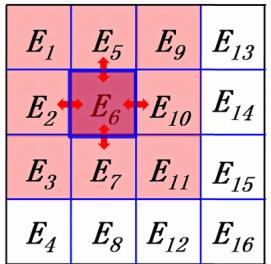
\includegraphics[keepaspectratio,alt={image}]{images/db5936d38db37ce8ac9f39d176bc0c25e311f3f6117a82f69e798fe0e2571d8d.jpg}}

\pandocbounded{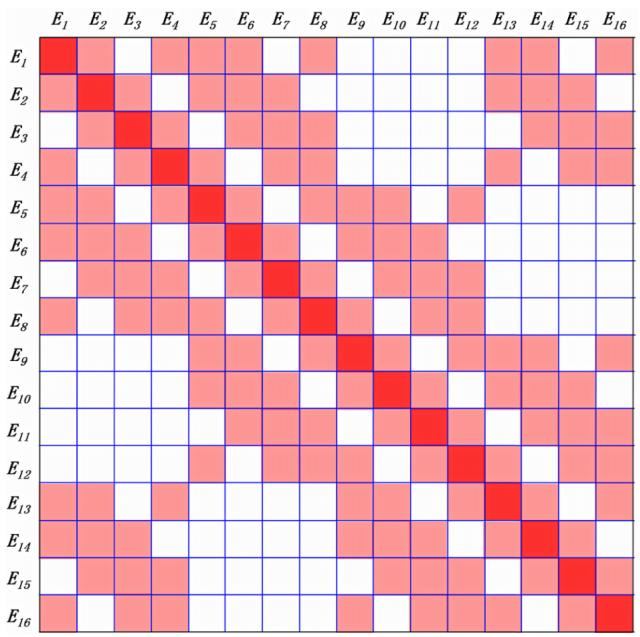
\includegraphics[keepaspectratio,alt={image}]{images/a67384afddbccac9fbf72c4b92567c5e37d537d43e8543b3c74612ec3932275b.jpg}}

\begin{enumerate}
\def\labelenumi{(\alph{enumi})}
\setcounter{enumi}{1}
\tightlist
\item
\end{enumerate}

FIG. 1. Partitioning of a domain into DG elements and the resulting
discretized Hamiltonian \(H ^ { \mathrm { D G } }\) . (a) Schematic
\(4 \times 4\) partition of a model 2D computational domain into 16
elements. (b) The DG Hamiltonian matrix
\(H ^ { \mathrm { D \bar { G } } }\) with its block sparsity pattern
resulting from such a partition. White represents zero blocks.

At the end of the ALB generation process, each element \(E _ { K }\) has
a collection of \(J _ { K }\) ALB functions, denoted by \{ K
\(\{ \bar { \varphi } _ { K , j } \} _ { j = 1 } ^ { J _ { K } }\)
j\}JKj=1. Each ALB is compactly supported on one element. ϕ ,The
complete collection of ALB functions

\[
\mathcal {A} = \left\{\varphi_ {K, j} \right\} _ {K = 1, j = 1} ^ {K = M, j = J _ {K}} \tag {1}
\]

forms an \(L ^ { 2 }\) orthonormal set over \(\Omega ,\) , i.e.,

\[
\left\langle \varphi_ {K, j}, \varphi_ {K ^ {\prime}, j ^ {\prime}} \right\rangle_ {\mathcal {T}} = \delta_ {K, K ^ {\prime}} \delta_ {j, j ^ {\prime}}, \tag {2}
\]

for
\(K , K ^ { \prime } = 1 , \ldots , M ; \ j = 1 , \ldots , J _ { K } ;\)
; and \(j ^ { \prime } = 1 , \ldots , J _ { K ^ { \prime } }\) ′. The ,
, . . . , , . . . , , . . . ,global Kohn-Sham states over Ω can be
expanded using the ALB functions as

\[
\psi_ {i} (x) = \sum_ {K = 1} ^ {M} \sum_ {j = 1} ^ {J _ {K}} c _ {i; K, j} \varphi_ {K, j} (x). \tag {3}
\]

Due to the fact that the ALB functions are discontinuous over the global
domain, whereas the Kohn-Sham states (and related physical quantities
such as the electron density) are continuous, the DG framework penalizes
discontinuities in these quantities across element surfaces.
Accordingly, the electronic free energy of a system with \(N _ { s }\)
occupied electronic states is written as

\[
\begin{array}{l} E _ {\text { free }} ^ {\mathrm{DG}} (\{\psi_ {i}, f _ {i} \}) = \sum_ {i = 1} ^ {N _ {s}} 2 f _ {i} \langle \nabla \psi_ {i}, \nabla \psi_ {i} \rangle_ {\mathcal {T}} + \langle V _ {\text { eff }}, \rho \rangle_ {\mathcal {T}} \\ + \sum_ {i = 1} ^ {N _ {s}} 2 f _ {i} \sum_ {I = 1} ^ {N _ {A}} \sum_ {\ell = 1} ^ {L _ {I}} \gamma_ {I, \ell} \left\langle b _ {I, \ell} (\cdot - R _ {I}), \psi_ {i} \right\rangle_ {\mathcal {T}} ^ {2} \\ - T _ {\mathrm{el}} S _ {\mathrm{el}} (\{f _ {i} \}) \\ - \sum_ {i = 1} ^ {N _ {S}} 2 f _ {i} \left\langle \left\{\left\{\nabla \psi_ {i} \right\} \right\}, \llbracket \psi_ {i} \rrbracket \right\rangle_ {\mathcal {S}} \\ + \alpha \sum_ {i = 1} ^ {N _ {s}} 2 f _ {i} \left\langle [   [ \psi_ {i} ]   ], [   [ \psi_ {i} ]   ] \right\rangle_ {\mathcal {S}}, \tag {4} \\ \end{array}
\]

where \(0 \leq f _ { i } \leq 1\) are the electronic occupation numbers
(specified via Fermi-Dirac smearing), \(V _ { \mathrm { e f f } }\)
denotes the effective potential (consisting of local pseudopotential,
Hartree, and exchange correlation contributions), the scalars
\(\gamma _ { I , \ell }\) and projector functions \(b _ { I , \ell }\) γ
,ℓcorrespond to the nonlocal ,ℓpseudopotential expressed in the
Kleinman-Bylander form,52 and \(T _ { \mathrm { e l } }\) and
\(S _ { \mathrm { e l } }\) correspond to the electronic temperature and
electronic entropy, respectively. The quantity is an adjustable αpenalty
parameter that ensures that Eq. (4) has a well-defined ground state free
energy.

Using the ALB functions to discretize the above expression for the free
energy and subsequently minimizing the discretized energy with respect
to the expansion coefficients \(c _ { i ; K , j }\) (as well as the
occupation numbers \(f _ { i } ) _ { \ast }\) , while maintaining the
orthonormality constraint on the orbitals, lead us to the discretized
version of the Euler--Lagrange equations. This takes the form of the
following eigenvalue problem:

\[
\sum_ {K ^ {\prime}, j ^ {\prime}} H _ {K, j; K ^ {\prime}, j ^ {\prime}} ^ {\mathrm{DG}} c _ {i; K ^ {\prime}, j ^ {\prime}} = \lambda_ {i} c _ {i; K, j}, \tag {5}
\]

with the discretized Hamiltonian operator expressible as

\[
\begin{array}{l} H _ {K, j; K ^ {\prime}, j ^ {\prime}} ^ {\mathrm{DG}} \\ = \Big (\frac {1}{2} \big \langle \nabla \varphi_ {K, j}, \nabla \varphi_ {K, j ^ {\prime}} \big \rangle_ {\mathcal {T}} + \big \langle \varphi_ {K, j}, V _ {\mathrm{eff}} \varphi_ {K, j ^ {\prime}} \big \rangle_ {\mathcal {T}} \Big) \delta_ {K, K ^ {\prime}} \\ \left. + \left(\sum_ {I, \ell} \gamma_ {I, \ell} \left\langle \varphi_ {K, j}, b _ {I, \ell} \right\rangle_ {\mathcal {T}} \left\langle b _ {I, \ell}, \varphi_ {K ^ {\prime}, j ^ {\prime}} \right\rangle_ {\mathcal {T}}\right) \right. \\ + \left(- \frac {1}{2} \left\langle [   [ \varphi_ {K, j} ]   ], \{\{\nabla \varphi_ {K ^ {\prime}, j ^ {\prime}} \} \} \right\rangle_ {S} \right. \\ + - \frac {1}{2} \left\langle \{\{\nabla \varphi_ {K, j} \} \}, [ [ \varphi_ {K ^ {\prime}, j ^ {\prime}} ] ] \right\rangle_ {S} \\ + \alpha \left\langle \llbracket \varphi_ {K, j} \rrbracket , \llbracket \varphi_ {K ^ {\prime}, j ^ {\prime}} \rrbracket \right\rangle_ {\mathcal {S}}). \tag {6} \\ \end{array}
\]

The matrix \(H ^ { \mathrm { D G } }\) can be naturally partitioned into
blocks based on the element indices. We will denote the
\(( K , K ^ { \prime } ) \mathrm { t h }\) matrix sub-block (of size
\(J _ { K } \times J _ { K ^ { \prime } } )\) as

\[
H _ {K; K ^ {\prime}} ^ {\mathrm{DG}} = H _ {K, j = 1, \dots , J _ {K}; K ^ {\prime}, j ^ {\prime} = 1, \dots , J _ {K ^ {\prime}}} ^ {\mathrm{DG}}. \tag {7}
\]

Since the ALB functions are compactly supported on their respective
elements, the block HDGK;K
\(H _ { K ; K ^ { \prime } } ^ { \mathrm { { D G } } }\) is non-zero
only when K and \(K ^ { \prime }\) refer to neighboring elements. This
situation is illustrated in Figure 1.

Further details on interpretation and computation of the various terms
described above as well as the significance of the parameter in
practical calculations can be found in αRefs. 21 and 23. Note that the
appearance of average and jump operators in Eqs. (4) and (6) is a
distinguishing feature of the interior penalty DG formulation of the
Kohn-Sham equations.

During the SCF iterations, the matrix \(H ^ { \mathrm { D G } }\) is
constructed using the most recent effective total potential
\(V _ { \mathrm { e f f } } .\) Following this, the electron density
needs to be computed from \(H ^ { \mathrm { D \bar { G } } }\) . So far,
this step has been achieved in the DGDFT code in two distinct ways. In
the first approach, the use of a parallel eigensolver (the ScaLAPACK
routine PDSYEVD) allows one to directly compute the eigenvalues and
eigenvectors of \(H ^ { \mathrm { D G } }\) . From these, the orbital
occupations \(\{ f _ { i } \} _ { i = 1 } ^ { N _ { s } }\) can be
computed via Fermi-Dirac smearing while the density matrix (also called
the Fermi matrix at finite electronic temperature) and the electron
density can be computed from the eigenvectors as

\[
P _ {K, j; K ^ {\prime}, j ^ {\prime}} = \sum_ {i = 1} ^ {N _ {s}} f _ {i} c _ {i; K, j} c _ {i; K ^ {\prime}, j ^ {\prime}}, \tag {8}
\]

\[
\rho (x) = 2 \sum_ {K = 1} ^ {M} \sum_ {j = 1} ^ {J _ {K}} \sum_ {j ^ {\prime} = 1} ^ {J _ {K}} \varphi_ {K, j} (x) \varphi_ {K, j ^ {\prime}} (x) P _ {K, j; K, j ^ {\prime}}. \tag {9}
\]

Eq. (9) shows that only the diagonal blocks of the density matrix need
to be computed to evaluate the electron density. Note that the
calculation of these blocks can be done individually on each element.

The second approach involves the use of the PEXSI technique to directly
compute the density matrix elements, without going through the
intermediate eigenvalues and eigenvectors. The electron density can be
evaluated subsequently from Eq. (9) using the diagonal blocks of the
density matrix, while the computation of forces requires computation of
the non-diagonal blocks corresponding to the sparsity pattern of
\(H ^ { \mathrm { D G } , 2 2 , \ d 3 8 }\)

Considering the limitations of each of the above approaches (as
described earlier), we now explore the option of using Chebyshev
polynomial filtered subspace iteration to compute the eigenvalues and
eigenvectors of \(\mathsf { \bar { H } } ^ { \mathrm { D G } }\) .

\section{B. Chebyshev polynomial filtered subspace iteration within
DGDFT}\label{b.-chebyshev-polynomial-filtered-subspace-iteration-within-dgdft}

Subspace iteration is a generalization of the classical power method for
computing the dominant eigenpair of a matrix.53,54 The standard subspace
iteration can be used to obtain an approximation to the invariant
subspace associated with the largest few eigenvalues. In Kohn-Sham DFT,
the invariant subspace of interest is the one associate with the
occupied states (and possibly a few unoccupied states above the Fermi
level)55,56 which do not correspond to the dominant eigenvalues of the
Kohn-Sham Hamiltonian.

A Chebyshev polynomial \(p _ { m } ( \lambda )\) can be constructed to
map eigenvalues at the low end of the spectrum (corresponding to the
occupied states) of \(H ^ { \mathrm { D G } }\) to the dominant
eigenvalues of \(p _ { m } ( H ^ { \mathrm { D G } } )\) . The
exponential growth property of the Chebyshev polynomials outside the
region {[}−1 1{]} can be used to ensure ,that the wanted part of the
spectrum (i.e., the occupied states in ground state electronic structure
calculations) can be magnified while the unwanted part (corresponding to
the unoccupied states) is damped in comparison.57--59 Applying subspace
iteration to \(p _ { m } ( H ^ { \mathrm { D G } } )\) yields the
desired invariant subspace. Within each iteration, the multiplication of
\(p _ { m } ( H ^ { \mathrm { D G } } )\) with a block of vectors can be
carried out by using the threeterm recurrence satisfied by Chebyshev
polynomials. The application of the Chebyshev polynomial filtered
subspace iteration (CheFSI) technique for computing the occupied
eigenspace of the Kohn-Sham operator was introduced in Refs. 43 and 44.
Within the SCF iteration framework, this methodology can be thought of
as a form of nonlinear subspace iteration in the sense that the approach
de-emphasizes the accurate solution of the intermediate linearized
Kohn-Sham eigenvalue problems on every SCF step. With the progress of
the SCF iterations, the approximate Hamiltonian approaches the
self-consistent one and the span of the (approximately) computed
eigenvectors approaches the converged occupied subspace simultaneously.
This particular feature of CheFSI has some bearing on the way it is
implemented within the DG framework, as explained later.

The main desirable features of CheFSI which make it suitable for
application to large-scale electronic structure problems are the
following: (1) It is a block method in which \(H ^ { \mathrm { D G } }\)
can be multiplied with a block of vectors simultaneously. This
additional level of concurrency allows the algorithm to achieve better
parallel scalability compared to standard Krylov subspace methods such
as the Lanczos algorithm. (2) Compared to other Krylov subspace methods,
it performs fewer Rayleigh-Ritz calculations in which a projected
subspace eigenvalue problem is solved. The Rayleigh-Ritz procedure is
often the computational bottleneck when the number of eigenvalues to be
computed is relatively large.

The key steps in a CheFSI cycle (see Algorithm 1 for details) are an
application of the Chebyshev polynomial filter on a block of vectors,
subsequent orthonormalization of the filtered block, a Rayleigh-Ritz
step, and finally a so-called subspace rotation step.43,45 Together, the
last three steps will be referred to as solving the subspace problem.
Note that the Rayleigh-Ritz and subspace rotation steps are useful for
explicitly obtaining the (approximate) occupied eigenpairs of the
Hamiltonian from the filtered subspace. We will now elaborate on various
important aspects of our implementation of these steps within DGDFT.

\section{\texorpdfstring{1. The multiplication of \(H ^ { \tt D G }\)
with a block of
vectors}{1. The multiplication of H \^{} \{ \textbackslash tt D G \} with a block of vectors}}\label{the-multiplication-of-h-tt-d-g-with-a-block-of-vectors}

One of the key computational steps of the CheFSI method is to perform
\(Y = p _ { m } ( H ^ { \mathrm { D G } } )\) X . This step requires an
efficient and scalable implementation of multiplying
\(\bar { H } ^ { \mathrm { D G } }\) with a block of vectors.
Additionally, computation of the action of the Hamiltonian matrix on
vectors is required for estimating the spectral bounds of the
Hamiltonian via the Lanczos algorithm as well as during the
Rayleigh-Ritz step (see Algorithm 1).

Given a block of vectors X consisting of columns
\(\left\{ x _ { i } \right\} _ { i = 1 } ^ { N _ { s } } ,\) the
multiplication of \(H ^ { \mathrm { D G } }\) with a subset of these
columns \(x _ { i _ { 1 } , \dots , i _ { 2 } } ,\) with
\(1 \leq i _ { 1 } \leq i _ { 2 } \leq N _ { s }\) , can be written as

\[
y _ {i _ {1}, \dots , i _ {2}; K, j} = \sum_ {K ^ {\prime}, j ^ {\prime}} H _ {K, j; K ^ {\prime}, j ^ {\prime}} ^ {\mathrm{DG}} x _ {i _ {1}, \dots , i _ {2}; K ^ {\prime}, j ^ {\prime}}, \tag {10}
\]

where \(K , K ^ { \prime } = 1 , \ldots , M\) and
\(j = 1 , \dotsc , J _ { K } , j ^ { \prime } = 1 , \dotsc , J _ { k ^ { \prime } } .\)
. , , . .Using the fact that
\(H _ { K ; K ^ { \prime } } ^ { \mathrm { { D G } } }\) , . . . , ,is
non-zero only for \(K ^ { \prime } \in { \mathcal { N } } ( K )\) ,
i.e., the neighboring elements of the Kth element, we may rewrite this
as

\[
y _ {i _ {1}, \dots , i _ {2}; K, j} = \sum_ {K ^ {\prime} \in \mathcal {N} (K)} H _ {K; K ^ {\prime}} ^ {\mathrm{DG}} x _ {i _ {1}, \dots , i _ {2}; K ^ {\prime}, j ^ {\prime}}. \tag {11}
\]

Thus, the portion of the resulting set of vectors
\(y _ { i _ { 1 } , \dots , i _ { 2 } }\) that is associated with the
element K can be written as

\[
y _ {i _ {1}, \dots , i _ {2}; K} = \sum_ {K ^ {\prime} \in \mathcal {N} (K)} H _ {K; K ^ {\prime}} ^ {\mathrm{DG}} x _ {i _ {1}, \dots , i _ {2}; K ^ {\prime}}. \tag {12}
\]

Since the individual blocks
\(H _ { K ; K ^ { \prime } } ^ { \mathrm { { D G } } }\) and
\(\lambda _ { i _ { 1 } , . . . , i _ { 2 } ; K ^ { \prime } }\) are
dense, ,\ldots,Eq. (12) can be computed as the sum of a series of
matrix-matrix products (i.e., GEMM operations in Level-3 BLAS). Further,
since the above operation can be carried out independently over the
various columns of X, it is natural to take advantage of the manifestly
parallel nature of the problem by distributing the columns among
separate processing elements in an appropriate manner.

The data distribution of the various quantities involved in Eq. (12) is
important in deciding how the operation can be carried out in practice.
As explained in Ref. 23, the DGDFT code uses a two-level parallelization
strategy implemented via Message Passing Interface (MPI) to handle
inter-process communication. At the coarse grained level, work is
distributed among processors by elements, leading to inter-element
parallelization. Further, within each element, the work associated with
construction of the local portions of the DG Hamiltonian, evaluation of
the electron density, and the ALB generation process is parallelized
leading to intra-element parallelization. The processors are partitioned
into a two-dimensional logical process grid with a column major order
(Fig. 2). We will refer to this layout of the MPI processes as the
global process grid. For the sake of

ALGORITHM 1. CheFSI cycle.

Input: Matrix \(H ^ { \mathrm { D G } } ,\) starting vector block X ,
filter order m

\begin{enumerate}
\def\labelenumi{\arabic{enumi}.}
\item
  Compute lower bound \(b _ { \mathrm { l o w } }\) using previous Ritz
  values and the upper bound \(b _ { \mathrm { u p } }\) using a few
  steps of the Lanczos algorithm.
\item
  Perform Chebyshev polynomial filtering, i.e., compute
  \(\tilde { Y } = p _ { m } ( H ^ { \mathrm { D G } } ) X\) with
  \([ b _ { \mathrm { l o w } } , b _ { \mathrm { u p } } ]\) mapped to
  {[}−1 1{]}.
\item
  Orthonormalize columns of Y˜ : Set
  \(S = \tilde { Y } ^ { T } \tilde { Y }\) , compute
  \(U ^ { T } U = S ,\) and solve
  \({ \hat { Y } } U = { \tilde { Y } } .\)
\item
  Rayleigh-Ritz step: Compute the projected subspace matrix
  \(\hat { H } = \hat { Y } ^ { T } H ^ { \mathrm { D G } } \hat { Y }\)
  and solve the eigenproblem
  \(\begin{array} { r } { \hat { H } Q = Q D . } \end{array}\)
\item
  Perform a subspace rotation step
  \(X _ { \mathrm { n e w } } = { \hat { Y } } Q .\)
\end{enumerate}

Output: Vector block \(X _ { \mathrm { n e w } }\) (approximate
eigenvectors) and Ritz values D (approximate eigenvalues).

M = Number of DG elements

{\def\LTcaptype{none} % do not increment counter
\begin{longtable}[]{@{}|l|l|l|l|l|@{}}
\toprule\noalign{}
\endhead
\bottomrule\noalign{}
\endlastfoot
\hline
1 & P\_e+1 & 2P\_e+1 & ... & (M-1)P\_e+1 \\
\hline
2 & P\_e+2 & 2P\_e+2 & ... & (M-1)P\_e+2 \\
\hline
3 & P\_e+3 & 2P\_e+3 & ... & (M-1)P\_e+3 \\
\hline
... & ... & ... & ... & ... \\
\hline
P\_e & 2P\_e & 3P\_e & ... & MP\_e \\
\hline
\end{longtable}
}

FIG. 2. Two-level parallelization scheme within DGDFT: the number of DG
elements is M and each element has \(P _ { e }\) processors dedicated to
it, making the total number of processors
\(P _ { \mathrm { t o t } } = M \times P _ { e }\) .

discussion, we assume here that the total number of MPI processes (in
the global process grid) is
\(P _ { \mathrm { t o t } } = M \times P _ { e } ,\) , so that there are
\(P _ { e }\) processes assigned to each of the M elements.
Specifically, the processes with MPI ranks \(( K - 1 ) P _ { e } + 1\)
to \(K P _ { e } \left( K = 1 , \ldots , M \right)\) are in the Kth
global column processor group, and they work on the element
\(E _ { K }\) at the level of intra-element parallelization.
Analogously, the ith global row processor group consists of the
processes with MPI ranks
\(i , P _ { e } + i , . . . , ( M - 1 ) P _ { e } + i ( i = 1 , . . . , P _ { e } )\)
. Any process in the , , . . . , , . . . ,global process grid can be
referred to by its row and column indices (I K ) in the process grid,
with \(I = 0 , \ldots , P _ { e } - 1\) and \(K = 0 , \ldots , M - 1\) .

, . . . ,The two-level parallelization scheme within DGDFT allows (12)
to be evaluated efficiently and in a scalable manner. A given block of
vectors X is distributed at the inter-element parallelization level in a
manner consistent with the element-wise partition suggested by Eq. (12),
and it is further distributed by its columns (i.e., Kohn-Sham states) at
the intra-element parallelization level. In other words, for a block of
vectors of size \(N _ { b } \times N _ { s }\) (with
\(\begin{array} { r } { N _ { b } = \sum _ { k = 1 } ^ { M } J _ { K } , \mathrm { i . e . } } \end{array}\)
, the total number of basis functions in use and \(N _ { s }\) denoting
the total number of Kohn-Sham states), the MPI process with row and
column indices (I K) holds a block of size
\(\begin{array} { r } { J _ { K } \times \lfloor \frac { N _ { s } } { P _ { e } } \rfloor } \end{array}\)
, and evaluates this portion of the result (i.e., left hand side of Eq.
(12)). In DGDFT, the matrix \(H ^ { \mathrm { D G } }\) is stored
element-wise, i.e., all \(P _ { e }\) processes in a given process grid
column assigned \(H _ { K ; K } ^ { \mathrm { { D G } } } ,\) articular
element K store all non-zero blocks of the form′. Hence, for a given
process, evaluation of (12) only incurs nearest neighbor communication
within each process grid row so that blocks of the form
\(x _ { i _ { 1 } , \dots , i _ { 2 } ; K ^ { \prime } }\) (with
\(i _ { 1 } , i _ { 2 }\) ,\ldots, ,corresponding to the start and end
indices of the block of states that the process is working on, and
\(K ^ { \prime }\) corresponding to its nearest neighbor elements) may
be obtained.

The strategy of employing a process grid avoids costly global
communication and restricts all communication to individual row and
column process grids. Additionally, the block nearest-neighbor type
sparsity structure of the Hamiltonian matrix results in further
reduction in communication volume. As demonstrated later, these factors
result in a particularly well scaling matrix-vector product routine for
DGDFT. In contrast, expressing \(H ^ { \mathrm { D G } }\) and the block
of vectors to be multiplied as dense matrices and the subsequent direct
use of parallel dense linear algebra routines (PBLAS,60 for example) for
carrying out the matrix-vector product operation would have incurred a
higher computational cost and also significantly degraded the
scalability of the computation.

\section{2. Parallel solution of the subspace
problem}\label{parallel-solution-of-the-subspace-problem}

The various steps involved in solving the subspace problem all require
dense linear algebra operations. For example, given the Chebyshev
polynomial filtered block of vectors
\(\tilde { Y } = p _ { m } ( H ^ { \mathrm { D G } } ) X\) , we need to
orthonormalize this block of vectors so as to obtain an orthonormal
basis for the (approximate) occupied subspace. We carry out this
operation by computing the overlap matrix
\(S = \tilde { Y } ^ { \tilde { T } } \tilde { Y }\) , computing the
Cholesky factorization of S as \(S = U ^ { T } U\) , and then using the
Cholesky factor to solve the equation
\({ \hat { Y } } U = { \tilde { Y } }\) . The resulting block of vectors
\(\hat { Y }\) is then orthonormal. The cost of these operations grows
cubically with respect to the number of atoms involved in the
simulation. Once the number of occupied states exceeds a few hundred, it
becomes necessary to parallelize these operations so as to reduce the
computational wall times. We use the parallel dense linear algebra
routines in the PBL \(\mathbf { A } \mathbf { S } ^ { 6 0 }\) and
ScaLAPACK29,30 software libraries to do this.

PBLAS and ScaLAPACK routines employ a twodimensional block-cyclic data
distribution over a process grid for their operations. We will refer to
this process grid as the linear algebra process grid. Since the
performance of some of the required routines (particularly, those
involved with eigenvalue computation and Cholesky factorization) tends
to stagnate (or sometimes, even deteriorate) quite easily if too many
processes are in use, we typically use only the first row of processes
of the global process grid to set up the linear algebra process grid for
the problems of moderate size. Thus, the number of processes in the
linear algebra process grid typically equals the number of DG elements
in use. As the system size grows bigger, we include additional rows of
processors in the global processor grid in the linear algebra process
grid to reduce the cost of dense linear algebra operations.

Before the sequence of dense linear algebra operations can be initiated,
the vector block that contains the product of
\(p _ { m } ( H ^ { \mathrm { D G } } )\) and X must be redistributed
over the linear algebra process grid from its distribution over the DG
elements. We have implemented routines for seamlessly inter-converting
between a block of vectors distributed over the DG elements to one
distributed over the linear algebra process grid, at relatively low
communication cost.23 In our experience, this step takes no more than 0
1\% of the total time spent in the .CheFSI routine, even for the largest
systems considered here.

The original Chebyshev filtering method presented in Refs. 43 and 44
employs a QR factorization or the DGKS algorithm61 for
orthonormalization. Here, we have used the faster (but sometimes less
stable) Cholesky factorization method instead. We have found that this
speeds up the orthonormalization by a factor of 2--3 in most cases with
no problematic side effects.

With the orthonormalized and filtered block of vectors
\({ \hat { Y } } ,\) the next step is to compute the projection of
\(H ^ { \mathrm { D G } }\) onto the occupied subspace:
\(\hat { H } = \hat { Y } ^ { T } ( H ^ { \mathrm { D } \mathrm { \bar { G } } } \hat { Y } )\)
. This step requires the vector block \(\hat { Y }\) distributed over
the linear algebra process grid to be redistributed over the DG
elements, so that the action of \(H ^ { \mathrm { D G } }\) on it can be
computed. Once again, this data redistribution step takes no more than 0
1\% of the total time .spent in the CheFSI routine, even for the largest
problems considered here.

After diagonalizing the projected matrix \(\hat { H } ,\) the resulting
block of eigenvectors Q can be used to compute the final results of one
CheFSI cycle as \(X _ { \mathrm { n e w } } = { \hat { Y } } Q .\) . Eq.
(8) can now be used to compute the diagonal blocks of the density matrix
locally on each element, by using the eigenvector coefficients in
\(X _ { \mathrm { n e w } }\) . The corresponding Ritz values
\(\Lambda _ { i }\) can be used for adjusting the polynomial filter
bounds as well as computing the Fermi energy and occupation numbers.

\section{3. Alignment of eigenvectors with current
basis}\label{alignment-of-eigenvectors-with-current-basis}

What distinguishes DGDFT from traditional Kohn-Sham DFT solvers is the
change of the basis set in each SCF cycle. This change has implications
for the way we prepare the starting vectors for CheFSI on every SCF
step. Conventionally, the input to CheFSI at the ith SCF cycle is chosen
to be the approximate invariant subspace computed at the (i − 1)th SCF
step.43,45 However, since the basis set changes from one SCF cycle to
the next in DGDFT, the eigenvector coefficients computed in a given SCF
cycle relative to the basis of that cycle are not applicable to
subsequent SCF cycles with different bases. In practice, the change of
basis from one SCF cycle to the next becomes smaller as self-consistency
is approached; however, as we show below, the change is sufficiently
large to require explicit accommodation to minimize CheFSI iterations.

Figure 3 shows that even for a simple system containing a few hydrogen
atoms, a naive implementation of CheFSI, which simply uses the
eigenvector coefficients computed in the previous SCF cycle as the
starting guess for the current SCF cycle, fails to converge in even
\(4 5\) iterations (green curve), whereas a direct diagonalization of
\(H ^ { \mathrm { D G } }\) via ScaLAPACK results in SCF convergence
(blue curve) in less than 20 SCF iterations. To address this problem, we
may perform several cycles of CheFSI in every SCF step to compensate for
the poor initial approximation provided by the coefficients of the
previous SCF step. This strategy produces results closer to those
produced by exact diagonalization in each SCF cycle (black curve) but
repeating the CheFSI cycle multiple times on every SCF step increases
the overall computational cost of the method.

\pandocbounded{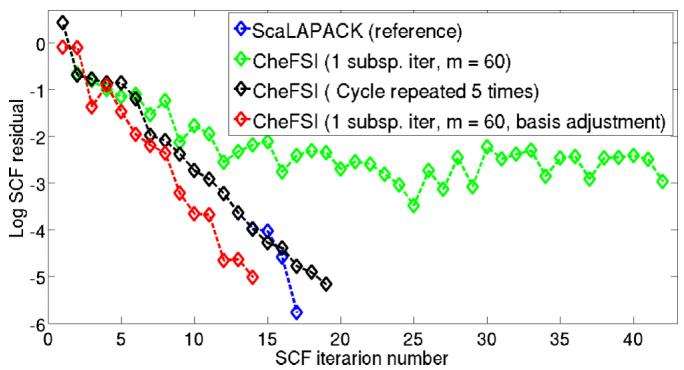
\includegraphics[keepaspectratio,alt={image}]{images/1b14fd3d3471f094ebac33434961c57f6bed3b54b96d1aff2b095d0d0be3b4a6.jpg}}

FIG. 3. SCF convergence of normalized electron density residual for
different variants of CheFSI within DGDFT (naive implementation,
multiple cycles, and eigenvector re-alignment to adjust for evolving
basis set) for a simple system containing a few hydrogen atoms.
Reference ScaLAPACK results are also presented.

Since the basis in a given SCF iteration is distinct from that of the
previous, with distinct span, the eigenvectors of the previous SCF
iteration cannot be expressed in terms of the basis of the current SCF
iteration without approximation. For optimality, we choose the best
approximation in the \(\ell ^ { 2 }\) norm, ℓwhich, by virtue of the
orthonormality of the DG basis, is readily obtained by \(\ell ^ { 2 }\)
projection. Specifically, if \(X ^ { ( i ) }\) denotes an
\(N _ { b } \times N _ { s }\) ℓblock of vector coefficients (where
\(N _ { b }\) denotes the total number basis functions in use and
\(N _ { s }\) denotes the number of Kohn-Sham states) computed by CheFSI
on a given SCF step, and \(V ^ { i }\) denotes an
\(N _ { r } \times N _ { b }\) block of basis vectors corresponding to
the ALB functions sampled on an \(N _ { r }\) -dimensional real-space
grid (consisting of Gauss-Lobatto integration points, for example, Ref.
21), then the starting point for the CheFSI method on SCF step i + 1 is
given by

\[
X ^ {(i + 1)} = (V ^ {i + 1}) ^ {T} V ^ {i} X ^ {(i)}. \tag {13}
\]

Since the ALB functions and the eigenvector coefficients
\(X ^ { ( i ) }\) and \(X ^ { ( i + 1 ) }\) are all distributed
DG-element-wise \(( \mathrm { i } . \mathrm { e } . , X ^ { ( i ) }\) ,
for example, is represented as M blocks
\(X _ { K } ^ { ( i ) } ; K = \dot { 1 } , \ldots , M\) stacked
column-wise), this becomes

\[
X ^ {(i + 1)} = \sum_ {K = 1} ^ {M} \left((V ^ {i + 1}) ^ {T} V ^ {i}\right) _ {K} (X ^ {(i)}) _ {K}. \tag {14}
\]

Further noting that ALB functions from different elements are orthogonal
to each other due to disjoint supports, we may rewrite the above as

\[
X _ {K} ^ {(i + 1)} = (V _ {K} ^ {i + 1}) ^ {T} V _ {K} ^ {i} (X _ {K} ^ {(i)}), \tag {15}
\]

with \(V _ { K } ^ { i }\) and \(V _ { K } ^ { i + 1 }\) denoting the
matrix representation of ALB functions originating from the element K on
SCF steps i and \(i + 1\) , respectively. Eq. (15) can be evaluated
locally on each element by means of two matrix-matrix multiplications.
As shown by the red curve in Figure 3, this extra step of realigning
results in SCF convergence with a rate comparable to that of exact
diagonalization.

In all the calculations presented here, this extra step of aligning the
wavefunction coefficients was always carried out from SCF step 2
onwards. The overhead due to this step is minimal (typically less than 0
1\% of the total time spent on .a CheFSI cycle) and does not grow with
system size since larger systems employ more elements and the
re-alignment calculation is carried out locally on each element.

A flowchart summarizing the various steps involved in the DG-CheFSI
method is presented in Figure 4.

\pandocbounded{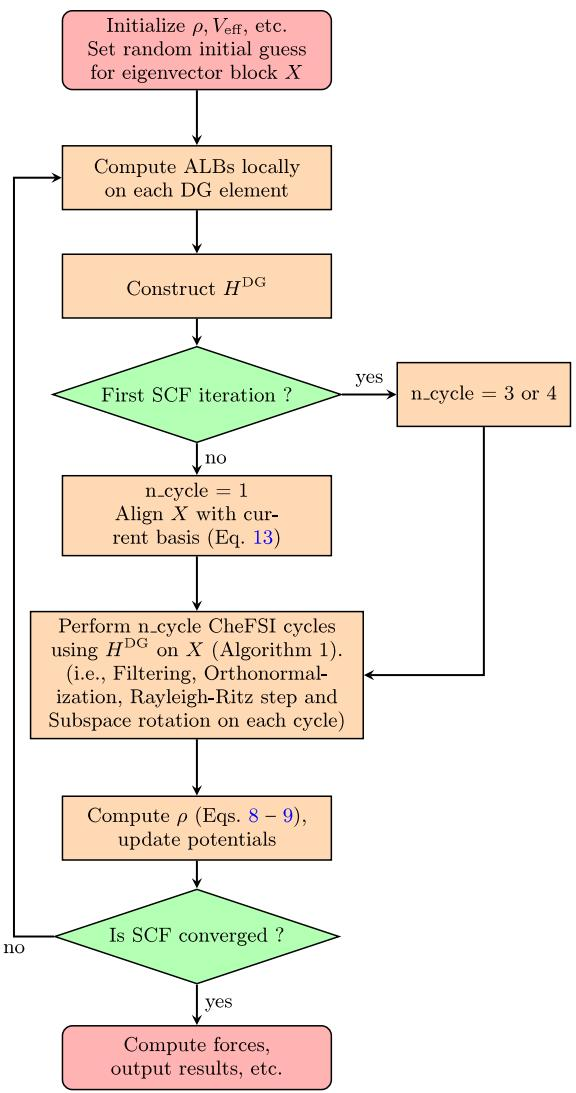
\includegraphics[keepaspectratio,alt={image}]{images/a53aefc5c02ae952aeeb039935d8beded7028109cddc77f1d0c644ef01374331.jpg}}

FIG. 4. Flowchart depicting the various steps of CheFSI within DGDFT.
Typically, 3 or 4 CheFSI cycles are applied on the first SCF step when
starting from a random guess for the eigenvector block X.

\section{4. Complexity analysis}\label{complexity-analysis}

For the purpose of this discussion, we let \(N _ { b }\) denote the
total number basis functions in use (i.e.,
\(\begin{array} { r } { N _ { b } = \sum _ { K = 1 } ^ { M } J _ { K } ) } \end{array}\)
and we let \(N _ { s }\) denote the number of Kohn-Sham states. Further,
we let \(N _ { g }\) represent the total number of real-space grid
points gin use, with \(N _ { g } / M\) grid points used for storing each
ALB g/locally within its associated element, with M elements. The
quantities \(\frac { N _ { b } } { M }\) and
\(\frac { N _ { g } } { M }\) then correspond to the number of ALB
functions per element and number of real-space grid points per element,
respectively, and are constants for a particular simulation and accuracy
level.

As explained above, the CheFSI approach mainly involves the application
of the Chebyshev polynomial filter on a block of vectors and subsequent
solution of the subspace problem. Within the DG framework, there is an
additional step of aligning the DG coefficients of the Kohn-Sham states
from one SCF step to the next. Regardless of the basis set in use (e.g.,
finite elements, planewaves, or ALB functions), the subspace problem
solution scales as
\(O ( N _ { b } N _ { s } ^ { 2 } + N _ { s } ^ { 3 } )\) due to the
requirement of dense matrix multiplications.43

Let us now focus on the polynomial filtering step. This involves
computing the product of the Hamiltonian matrix with the block of
Kohn-Sham states. After the generation process of the ALB functions (a
step which incurs a memory cost of \(O ( N _ { g } N _ { b } / M )\) on
every element), the memory cost associated with storage of the
coefficients of Kohn-Sham states in terms of the ALB functions is
\(O \left( N _ { b } N _ { s } + N _ { b } \frac { N _ { g } } { M } \right)\)
This contrasts with the storage cost of
\(O ( N _ { g } \dot { N } _ { s } )\) that would be grequired by finite
differences, finite elements, or planewave methods using the same number
of real-space grid points. In this sense, the use of ALB functions can
be seen as a systematically improvable compressed format for storing the
Kohn-Sham states. In practice, the number of ALB functions per element
\(N _ { b } / M\) is at most a few hundreds and this number /is usually
far exceeded by the number of Kohn-Sham states \(N _ { s } ,\) in large
calculations. Further \(N _ { b } / N _ { s }\) is typically 2--20.
Hence, once the ALB functions have been generated, there is overall less
memory cost involved in storing the Kohn-Sham states using the ALB
functions.

As explained earlier (Section II B 1, Eq. (11)), multiplying the block
sparse matrix \(H ^ { \mathrm { D G } }\) with the block of Kohn-Sham
states involves a few dense matrix multiplications of small blocks (of
size \(\frac { N _ { b } } { M } \times \frac { N _ { b } } { M } )\)
coming from \(H ^ { \mathrm { D G } }\) , with blocks (of size
\(\frac { N _ { b } } { M } \times N _ { s } \times\) coming from the
coefficients of the Kohn-Sham states, for each DG element. If there are
\(c _ { N }\) such multiplications to be carried out for each element
(this being related to the number of nearest neighbors of elements), the
total cost for the application of one step of the polynomial filter is
proportional to

\[
c _ {\mathcal {N}} \left(\frac {N _ {b}}{M}\right) ^ {2} N _ {s} M = O (N _ {s} M), \tag {16}
\]

since \(\frac { N _ { b } } { M }\) is a constant. Splitting this
calculation into the respective M elements therefore incurs a
computational cost of \(O ( N _ { s } )\) on every element. Note that,
in contrast, this computation using finite differences or finite
elements would have a complexity of \(O ( N _ { s } N _ { g } )\) in
total and is likely to incur a greater computational cost.

Finally, the step of aligning the Kohn-Sham states with the current
basis set on every SCF step (Eq. (14)) incurs a cost that is
proportional to

\[
\left(\frac {N _ {b}}{M}\right) ^ {2} \frac {N _ {g}}{M} + \left(\frac {N _ {b}}{M}\right) ^ {2} N _ {s} = \mathcal {O} (N _ {s}), \tag {17}
\]

on every element.

In contrast to the computational complexity of the various steps
involved in the CheFSI approach, direct diagonalization of
\(\dot { H } ^ { \mathrm { D G } }\) involves a computational complexity
of \(O ( N _ { b } ^ { 3 } )\) while the PEXSI approach involves a cost
of
\(\begin{array} { r } { O \Big ( \big ( \frac { N _ { b } } { M } \big ) ^ { 3 } M ^ { \alpha _ { D } } \Big ) } \end{array}\)
(with \(\alpha _ { D } = 1 . 0 , 1 . 5 , 2 . 0\) for one-, two-, and
three-dimensional α . , . , .systems, respectively). Direct
diagonalization is more computationally intensive while the PEXSI
approach results in a larger prefactor, because of which both methods
result in longer wall times to solution compared to CheFSI for the full
range of system sizes considered here.

\section{III. RESULTS}\label{iii.-results}

In this section, we investigate the parallel scalability of the CheFSI
method and compare its performance with the existing ScaLAPACK and PEXSI
methods in DGDFT. Two prototypical systems have been used for our
calculations. The first, referred to as Li3D, consists of a
three-dimensional bulk lithium-ion electrolyte system originating from
the design of energy storage devices. Atoms of hydrogen, lithium,
carbon, phosphorus, oxygen, and fluorine, numbering 318 in total, are
present in this system. The second, referred to as Graphene2D, consists
of a two-dimensional sheet of graphene containing 180 carbon atoms.
These systems were chosen for their technological relevance as well as
the fact that KS-DFT calculations on large samples of these systems can
be challenging. Figure 5 shows the Li3D and Graphene2D systems along
with the first ALB from one of the DG elements of these systems.

In order to be able to work with larger system sizes, we have employed
multiple unit cells of these systems replicated along the coordinate
axes. Thus,
\(\mathrm { L i } 3 \mathrm { D } _ { 1 \times 2 \times 2 } ,\) for
example, refers to a system in which the 318-atom unit cell has been
replicated along Y and Z directions to produce a 1272- atom bulk system,
and similarly, Graphene \$ \{ 2 \mathrm { D } \_ \{ 4 \times 4 \} \}\$
refers to a graphene sheet containing 2880 atoms.

\pandocbounded{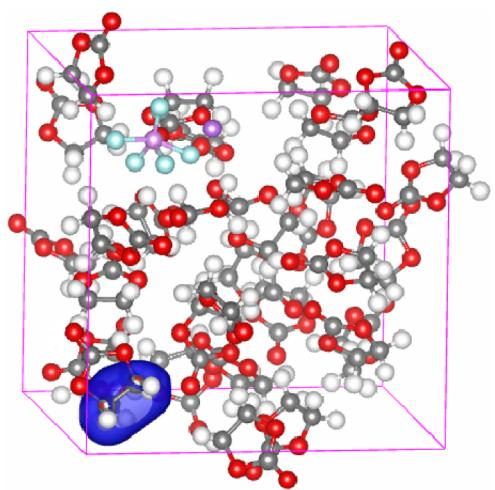
\includegraphics[keepaspectratio,alt={image}]{images/1b798553da6da6810c65405747eaea1d7d573b66bd77e78d9bcb285e235954a7.jpg}}

\begin{enumerate}
\def\labelenumi{(\alph{enumi})}
\tightlist
\item
\end{enumerate}

\pandocbounded{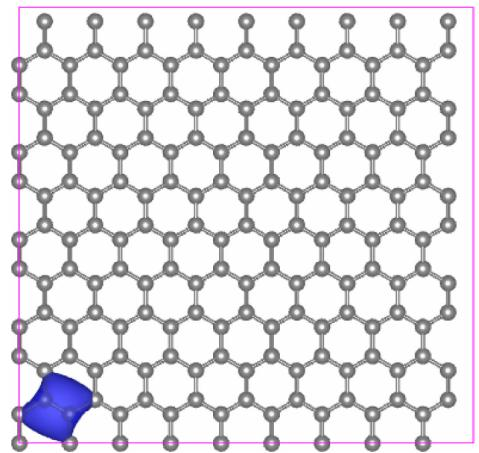
\includegraphics[keepaspectratio,alt={image}]{images/3e88904dc8e1c46385211115e63ba0919d5353cf6378fe856c543f6c5391ce3f.jpg}}

\begin{enumerate}
\def\labelenumi{(\alph{enumi})}
\setcounter{enumi}{1}
\tightlist
\item
\end{enumerate}

FIG. 5. Prototype 2D and 3D systems used for the computations in this
work. Larger sized systems were obtained by periodic replication of
these unit cells. Iso-surface of the first ALB from one of the DG
elements of these systems is also shown. (a) Bulk Li3D system containing
318 atoms. (b) Graphene2D system containing 180 atoms.

In what follows, we shall consider the time to solution. For the CheFSI
and ScaLAPACK diagonalization methods, this will refer to the wall clock
time that these methods require to compute the eigenvalues and
eigenvectors of \(H ^ { \mathrm { D G } }\) as well as the diagonal
blocks of the density matrix (via Eq. (8)), during a general SCF cycle.
For the PEXSI method, it will refer to the wall clock time that is
required to compute directly the density matrix corresponding to the
sparsity pattern of \(H ^ { \mathrm { D G } }\) . In order to have a
fair comparison between the methods, it is important to ensure that the
three methods show the same convergence rate over multiple SCF cycles.
This then allows the comparison between the methods to be carried out
with reference to the time to solution for one SCF cycle. Accordingly,
we have adjusted the Chebyshev polynomial filter order as well as the
various parameters used in PEXSI (such as the number of poles and the
number of chemical potential iterations), so that these methods converge
at least as fast as the reference ScaLAPACK calculations. Figure 6 shows
the convergence of all the three methods for the prototype systems in
use here.

For most of the calculations described here, the polynomial filter order
used was between 80 and 100. However, these employed relatively hard
pseudopotentials;62 lower filter orders may be expected to suffice for
softer pseudopotentials. Additionally, in practical molecular dynamics
and geometry optimization calculations, fewer SCF cycles are likely to
be required for the CheFSI method on every electronic relaxation step,
since the method will be able to make use of wavefunction extrapolation
(with re-alignment to account for the evolving basis set). Thus, the
performance of CheFSI in the context of MD simulations may be expected
to improve still further relative to the results of static calculations,
as presented here.

We have used the local density approximation for the
exchange-correlation functional with the parametrization described in
Ref. 63. Hartwigsen-Goedecker-Teter-Hutter pseudopotentials62,63 are
employed to remove inert core electrons from the computations. We have
typically employed 100--120 additional states in most calculations to
accommodate partial occupation. SCF convergence was accelerated by means
of Pulay's scheme64 or its periodic variant,65 and an electronic
temperature of 300 K was used in Fermi-Dirac occupation. To attain
chemical accuracy (i.e., error in the total energy less than
\(1 0 ^ { - 3 }\) Ha/atom relative to the fully converged result;
additionally we also ensured that the error in the atomic forces is less
than \(1 0 ^ { - 3 }\) Ha/bohr relative to the fully converged result),
the 318-atom bulk Li3D system was partitioned into
\(4 \times 4 \times 4\) elements, with 200 ALB functions per element,
giving ∼40 ALB functions per atom. Likewise, the 180-atom Graphene2D
system was partitioned into \(1 \times 6 \times 6\) elements, with 120
ALB functions per element, giving 24 ALB functions per atom.

\pandocbounded{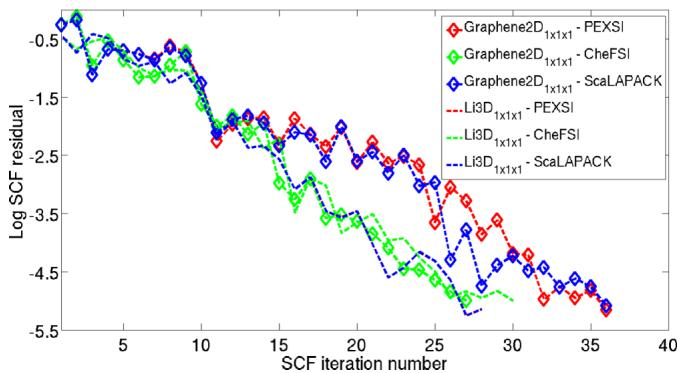
\includegraphics[keepaspectratio,alt={image}]{images/df333722dd91f2f809da81bb1f69fdf2fa014878768940360251157950187751.jpg}}

FIG. 6. SCF convergence of normalized electron density residual for two
prototypical systems using ScaLAPACK diagonalization, PEXSI, and CheFSI
methods.

All calculations described here were performed on the Edison platform at
the National Energy Research Scientific Computing (NERSC) center. Edison
has 5462 Cray XC30 nodes. Each node has 64 GB of memory and 24 cores
partitioned among two Intel Ivy Bridge processors, running at 2.4 GHz.
Edison employs a Cray Aries highspeed interconnect with Dragonfly
topology for inter-node communication.

\section{A. Scaling performance}\label{a.-scaling-performance}

We first investigate the strong scaling performance of CheFSI within the
DG framework and compare it against that of PEXSI and ScaLAPACK. For
this, we consider the systems
\(\mathrm { L i } 3 \mathrm { D } _ { 2 \times 2 \times 2 }\) (2544
atoms, 4536 Kohn-Sham states) and Graphene
\(2 \mathrm { D } _ { 6 \times 6 }\) (6480 atoms, 13 080 Kohn-Sham
states).

Figure 7 shows the wall time to solution (per SCF iteration) vs.~number
of computational cores employed. From

\pandocbounded{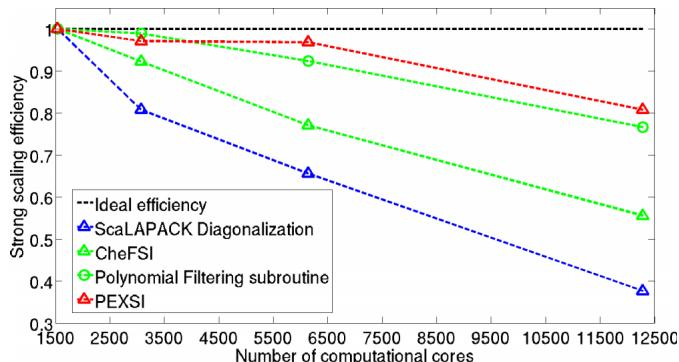
\includegraphics[keepaspectratio,alt={image}]{images/ad5bf58af6e164b25e37198d4ec876a9163e11ef5c5be96633600521d34ec16e.jpg}}

\begin{enumerate}
\def\labelenumi{(\alph{enumi})}
\tightlist
\item
\end{enumerate}

\pandocbounded{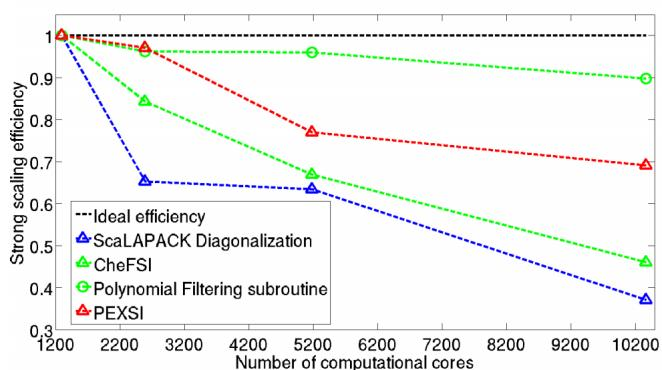
\includegraphics[keepaspectratio,alt={image}]{images/12230cd9af26bbe3a73b51f76a4cd7f606d4cba1b18bbf9d05d9266cca819bad.jpg}}

\begin{enumerate}
\def\labelenumi{(\alph{enumi})}
\setcounter{enumi}{1}
\tightlist
\item
\end{enumerate}

FIG. 7. Strong scaling efficiency of CheFSI in DGDFT, compared against
PEXSI and direct ScaLAPACK diagonalization. Scaling performance of the
filtering routine is also shown. (a)
\(\mathrm { L i } 3 \mathrm { D } _ { 2 \times 2 \times 2 }\) system
(2544 atoms). (b)
\(\mathrm { G r a p h e n e } 2 \mathrm { D } _ { 6 \times 6 }\) system
(6480 atoms).

the figures, it is evident that the overall strong scaling performance
of CheFSI lies in between that of PEXSI and direct ScaLAPACK
diagonalization. For the
\(\mathrm { L i } 3 \mathrm { D } _ { 2 \times 2 \times 2 }\) system,
the performance using 12 288 cores is at about 56\% efficiency (measured
against the result from 1500 cores), while for the
\(\mathrm { G r a p h e n e 2 D } _ { 6 \times 6 }\) system, using 10
368 processors, it is at about 46\% efficiency (measured against the
result from 1200 cores). It is interesting to note, however, that the
strong scaling performance of the filtering routine by itself is nearly
ideal, remaining close to 80\% efficiency for the
\(\mathrm { L i } 3 \mathrm { D } _ { 2 \times 2 \times 2 }\) case and
at about 90\% efficiency for the
\(\mathrm { G r a p h e n e } 2 \mathrm { D } _ { 6 \times 6 }\) case.
In particular, the performance of the filtering routine is better in the
2D system due to fewer neighboring elements and correspondingly less
communication required. The overall scaling performance of CheFSI,
therefore, is limited by the performance of the subspace problem
solution, whenever the total time for this step forms a significant
fraction of the total CheFSI time. For the systems here, the subspace
problem solution time was about 33\% of the total CheFSI time for the
\(\mathrm { L i } 3 \mathrm { D } _ { 2 \times 2 \times 2 }\) system
using 12 288 cores and 57\% of the total CheFSI time for the
\(\mathrm { G r a p h e n e } 2 \mathrm { D } _ { 6 \times 6 }\) system
using 10 368 cores. The larger fraction of time spent on the subspace
problem helps explain why the overall scaling performance of CheFSI is
somewhat lower for the 2D case here. These observations suggest possible
avenues for further improvement of the overall scaling performance of
CheFSI.

Next, we investigate the weak scaling performance of CheFSI within
DGDFT, i.e., the performance with increasing system size. We investigate
the following systems in 3D:
\(\mathrm { L i } 3 \mathrm { D } _ { 1 \times 1 \times 1 } , \mathrm { L i } 3 \mathrm { D } _ { 1 \times 1 \times 2 }\)
and \(\mathrm { L i } 3 \mathrm { D } _ { 1 \times 2 \times 2 }\) . The
system ,sizes have been doubled successively, and as a result, the
number of Kohn-Sham states involved (approximately) is doubled as well.
In 2D, we investigated the systems: Graphene
\(\mathrm { 2 D _ { 1 \times 1 } , G r a p h e n e 2 D _ { 2 \times 2 } }\)
, and \(\mathrm { G r a p h e n e } 2 \mathrm { D } _ { 4 \times 4 } .\)
. For ,these cases, the system sizes have been quadrupled successively,
and as a result, the number of Kohn-Sham states involved (approximately)
is quadrupled as well. As a measure of weak scaling performance, the
wall clock time to solution (per SCF iteration) is shown in Figure 8.
For each system, the number of computational cores was quadrupled
successively as sizes were doubled (Li3D) and quadrupled (Graphene2D)
successively.

On increasing the system size n fold, the number of DG elements used for
the calculation has to increase by the same factor to keep each local
calculation manageable and to maintain the same level of accuracy of
solution. Since the number of Kohn-Sham states involved also increases n
fold, there is an overall \(n ^ { 2 }\) factor increase in the time
required for applying the Chebyshev polynomial filter to all the states
involved \(\left( \mathrm { E q } . \ ( 1 6 ) \right)\) . Hence, if the
number of computational cores used for doing the larger calculation is
increased by a factor of s, the expected wall time for applying the
Chebyshev polynomial filter will change by a factor of \(n ^ { 2 } / s\)
. This observation should also hold for the total CheFSI /time, as long
as the time for solution of the subspace problem forms a small fraction
of the total CheFSI time. Thus, for the Li3D systems, the wall-times for
each system should ideally remain constant \(( n = 2 , s = 4 )\) , while
for the Graphene2D ,systems, an increase by a factor of 4 should be
observed \(( n = 4 , s = 4 )\) . Figure 8 shows that this expectation
holds ,reasonably well for the overall CheFSI time and particularly well
for the Chebyshev polynomial filter application time. For the Li3D
systems, the weak scaling efficiency of CheFSI is about 70\% using 3072
cores, while it is about 65\% using 4608 cores for the Graphene2D
systems. The performance of the polynomial filter application routine
for both these systems is close to 90\%. These results demonstrate again
the critical importance of an efficient, well scaling subspace solution
as system size increases beyond a few thousand atoms.

\pandocbounded{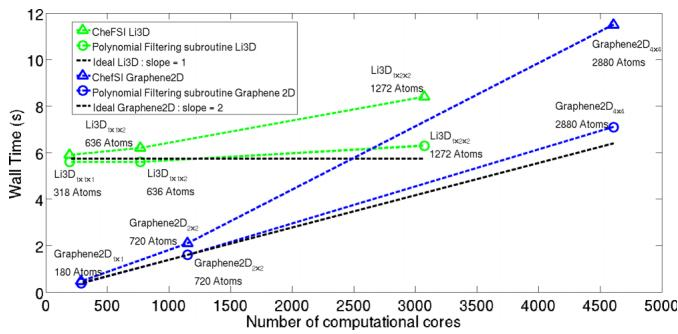
\includegraphics[keepaspectratio,alt={image}]{images/b32c274c64870fbe34edee6a70d24efcc16cfe866a7769dbba15655768446aa9.jpg}}

FIG. 8. Weak scaling performance of CheFSI in DGDFT. Performance of the
filtering routine is also shown.

\section{B. Benchmark calculations}\label{b.-benchmark-calculations}

As the final test of computational efficiency, we study the performance
of CheFSI on large benchmark systems and compare the wall time to
solution between CheFSI, direct ScaLAPACK diagonalization, and PEXSI. We
choose the \(\mathrm { L i } 3 \mathrm { D } _ { 3 \times 3 \times 3 }\)
and \(\mathrm { G r a p h e n e 2 D } _ { 8 \times 8 }\) systems for
this study. 13 824 computational cores were used for both systems. The
results are shown in Table I.

The results show that CheFSI is by far the fastest of all the three
approaches (up to more than an order of magnitude faster), particularly
for the bulk system. Even for the two-dimensional material system, a
geometry in which PEXSI is known to perform particularly well, CheFSI is
able to outperform with the same number of cores. Due to the good
scalability properties of PEXSI, the wall time for the
\(\mathrm { G r a p h e n e 2 D } _ { 8 \times 8 }\) system can be
brought down to be comparable to CheFSI (using 55 296 cores, for
instance), but overall CheFSI remains more economical in terms of
computational resources used (total CPU-hours, for example). We have
also observed that the timing results remain favorable for

TABLE I. Solution wall times per SCF step (rounded to nearest second)
for direct ScaLAPACK diagonalization, PEXSI, and CheFSI on 13 824
computational cores for two large systems.

{\def\LTcaptype{none} % do not increment counter
\begin{longtable}[]{@{}|l|l|l|l|@{}}
\toprule\noalign{}
\endhead
\bottomrule\noalign{}
\endlastfoot
\hline
System & ScaLAPACK & PEXSI & CheFSI \\
\hline
Li3D\_\{3\textbackslash times3\textbackslash times3\} & & & \\
\hline
8586 atoms & 3323 & 3784 & 170 \\
\hline
\textasciitilde15 000 states & & & \\
\hline
Graphene2D\_\{8\textbackslash times8\} & & & \\
\hline
11 520 atoms & 2473 & 426 & 105 \\
\hline
\textasciitilde23 200 states & & & \\
\hline
\end{longtable}
}

TABLE II. Wall times for various stages of the SCF cycle (rounded to
nearest second) with the DGDFT--CheFSI approach for two large systems
using 55 296 computational cores. The numbers in parentheses indicate
the wall time spent on the filtering step.

{\def\LTcaptype{none} % do not increment counter
\begin{longtable}[]{@{}|l|l|l|l|l|@{}}
\toprule\noalign{}
\endhead
\bottomrule\noalign{}
\endlastfoot
\hline
System & ALB generation & Hamiltonian update & CheFSI (filtering) &
Total SCF time \\
\hline
Li3D\_\{3\textbackslash times3\textbackslash times3\} & 11 & 3 & 76 (36)
& 90 \\
\hline
Graphene2D\_\{8\textbackslash times8\} & 5 & 4 & 66 (16) & 75 \\
\hline
\end{longtable}
}

CheFSI for smaller systems, such as those used in the scaling
performance studies.

In order to obtain an estimate of the SCF wall times achievable with the
DGDFT-CheFSI framework on largescale computational platforms, we studied
the \(\mathrm { L i } 3 \mathrm { D } _ { 3 \times 3 \times 3 }\) and
\(\mathrm { G r a p h e n e 2 D } _ { 8 \times 8 }\) systems using 55
296 computational cores. The results are shown in Table II.

It is apparent from the results in Table II that for these systems, the
largest fraction of the total SCF time is spent on the solution of the
subspace problem. Thus the cubic computational complexity associated
with the solution of the subspace problem starts to dominate as the
system size grows larger, beyond a few thousand atoms in the present
case.

\section{IV. CONCLUSION}\label{iv.-conclusion}

We have used Chebyshev polynomial filtered subspace iteration (CheFSI)
within the discontinuous Galerkin method to enable large-scale first
principles simulations of a wide variety of materials systems using
density functional theory. Due to a number of attractive features of the
DG Hamiltonian matrix, the implementation of CheFSI within the
discontinuous Galerkin framework allows the computation of the Kohn-Sham
eigenstates of the Hamiltonian to be carried out in a highly efficient
and scalable manner. By virtue of the limited spectral width of the DG
Hamiltonian matrix, relatively low polynomial orders suffice, reducing
the number of matrix-vector multiplies required, while the block-sparse
structure of the DG Hamiltonian facilitates efficient, parallel
implementation of each multiply. In addition, the strict locality and
orthonormality of the adaptive local basis facilitates realignment of
eigenvector coefficients from one SCF step to the next, as the basis is
optimized on-the-fly at each step. Taken together, these advantages
yield an accurate, systematically improvable electronic structure
method, applicable to metals and insulators alike, capable of simulating
thousands of atoms in tens of seconds per SCF iteration on large-scale
parallel computers.

In the near future, we aim to carry out large-scale quantum molecular
dynamics simulations of various materials systems using the DGDFT-CheFSI
technique. Of particular interest to us are accurate simulations of the
solid-electrolyte interphase (SEI) layer in lithium-ion batteries, and
we anticipate that the new methodology will enable accurate simulations
of unprecedented size.

While the current methodology can simulate a few thousand atoms in a few
tens of seconds per SCF iteration with planewave accuracy, to reach
further still, to 10 000 atoms or more with comparable efficiency, will
require a substantially more efficient and scalable solution of the
subspace problem. We aim to address this issue in future work. One
possible avenue for making this step more scalable is to replace the use
of Cholesky factorization and eigensolution (for the Rayleigh-Ritz step)
with operations which involve only parallel dense matrix multiplications
in the occupied subspace. Parallel dense matrix multiplication tends to
scale more favorably and therefore stands to relieve the scalability
bottleneck in the current approach. Yet another, more radical
possibility would be to dispense with the CheFSI methodology completely,
thus avoiding the Rayleigh-Ritz step. Computational techniques such as
\(\mathrm { F E A S T } ^ { 6 6 }\) or spectrum slicing67 might be used
to compute the spectrum of \(H ^ { \mathrm { D G } }\) instead. However,
compared to more conventional methods like CheFSI, these techniques are
likely more suitable for the next generation of computing platforms.49
An interesting avenue for future work, therefore, would be to
investigate whether such techniques can be made to yield significant
performance benefits on current parallel computing platforms for
physical systems of the types and sizes considered here.

Finally, comparison of the performance of DGDFT-CheFSI with other
massively parallel electronic structure codes, such as Qbox,68,69 is
another interesting avenue for research, which the authors are pursuing
presently.

\section{ACKNOWLEDGMENTS}\label{acknowledgments}

This work was performed, in part, under the auspices of the U.S.
Department of Energy by Lawrence Livermore National Laboratory under
Contract No.~DE-AC52- 07NA27344. The support for this work was provided
through Scientific Discovery through Advanced Computing (SciDAC) program
funded by the U.S. Department of Energy, Office of Science, Advanced
Scientific Computing Research and Basic Energy Sciences (A.S.B., L.L.,
W.H., C.Y., and J.E.P.), and by the Center for Applied Mathematics for
Energy Research Applications (CAMERA), which is a partnership between
Basic Energy Sciences and Advanced Scientific Computing Research at the
U.S. Department of Energy (L.L. and C.Y.). The authors thank the
National Energy Research Scientific Computing (NERSC) center for making
computational resources available to them. A.S.B. would like to thank
Meiyue Shao (Lawrence Berkeley Lab) for informative discussions and for
his help with improving the presentation of the manuscript. The authors
would also like to thank the anonymous reviewers for their comments
which helped in improving the manuscript.

1P. C. Hohenberg and W. Kohn, Phys. Rev.~136, 864 (1964).

2W. Kohn and L. J. Sham, Phys. Rev.~140, 1133 (1965).

3R. M. Martin, Electronic Structure: Basic Theory and Practical Methods,
1st ed.~(Cambridge University Press, 2004).

4J. Kohanoff, Electronic Structure Calculations for Solids and
Molecules: Theory and Computational Methods, 1st ed.~(Cambridge
University Press, 2006).

5M. C. Payne, M. P. Teter, D. C. Allan, T. A. Arias, and J. D.
Joannopoulos, Rev.~Mod. Phys. 64, 1045 (1992).

6G. Kresse and J. Furthmuller, Phys. Rev.~B 54, 11169 (1996).

7J. Pask and P. Sterne, Modell. Simul. Mater. Sci. Eng. 13, R71 (2005).

8E. Tsuchida and M. Tsukada, Phys. Rev.~B 52, 5573 (1995).

9H. Chen, X. Dai, X. Gong, L. He, and A. Zhou, Multiscale Model. Simul.
12, 1828 (2014).

10P. Suryanarayana, V. Gavini, T. Blesgen, K. Bhattacharya, and M.
Ortiz, J. Mech. Phys. Solids 58, 256 (2010).

11J. R. Chelikowsky, N. Troullier, K. Wu, and Y. Saad, Phys. Rev.~B 50,
11355 (1994).

12J. Chelikowsky, N. Troullier, and Y. Saad, Phys. Rev.~Lett. 72, 1240
(1994).

13S. Ghosh and P. Suryanarayana, preprint arXiv:1603.04334 (2016).

14A. Castro, H. Appel, M. Oliveira, C. Rozzi, X. Andrade, F. Lorenzen,
M. Marques, E. Gross, and A. Rubio, Phys. Status Solidi B 243, 2465
(2006).

15A. S. Banerjee, R. S. Elliott, and R. D. James, J. Comput. Phys. 287,
226 (2015).

16A. S. Banerjee, Density Functional Methods for Objective Structures:
Theory and Simulation Schemes, Ph.D.~thesis, University of Minnesota,
Minneapolis, 2013.

17W. Hehre, R. Stewart, and J. Pople, J. Chem. Phys. 51, 2657 (1969).

18J. C. Slater and G. F. Koster, Phys. Rev.~94, 1498 (1954).

19J. Soler, E. Artacho, J. Gale, A. Garca, J. Junquera, P. Ordejn, and
D. Snchez-Portal, J. Phys.: Condens. Matter 14, 2745 (2002).

20V. Blum, R. Gehrke, F. Hanke, P. Havu, V. Havu, X. Ren, K. Reuter, and
M. Scheffler, Comput. Phys. Commun. 180, 2175 (2009).

21L. Lin, J. Lu, L. Ying, and E. Weinan, J. Comput. Phys. 231, 2140
(2012).

22G. Zhang, L. Lin, W. Hu, C. Yang, and J. E. Pask, preprint arXiv:1510.
06489 (2015).

23W. Hu, L. Lin, and C. Yang, J. Chem. Phys. 143, 124110 (2015).

24W. Hu, L. Lin, and C. Yang, Phys. Chem. Chem. Phys. 17, 31397 (2015).

25D. N. Arnold, SIAM J. Numer. Anal. 19, 742 (1982).

26J. Kaye, L. Lin, and C. Yang, Commun. Math. Sci. 13, 1741 (2015).

27L. Lin and B. Stamm, preprint arXiv:1502.01738 (2015).

28L. Lin and B. Stamm, preprint arXiv:1603.04456 (2016).

29L. S. Blackford, J. Choi, A. Cleary, E. D'Azevedo, J. Demmel, I.
Dhillon, J. Dongarra, S. Hammarling, G. Henry, A. Petitet et al.,
ScaLAPACK Users' Guide (SIAM, 1997), Vol. 4.

30J. Choi, J. Demmel, I. Dhillon, J. Dongarra, S. Ostrouchov, A.
Petitet, K. Stanley, D. Walker, and R. C. Whaley, Applied Parallel
Computing Computations in Physics, Chemistry and Engineering Science
(Springer, 1995), pp.~95--106.

31S. Goedecker, Rev.~Mod. Phys. 71, 1085 (1999).

32D. Bowler and T. Miyazaki, Rep.~Prog. Phys. 75, 036503 (2012).

33N. D. Hine, P. D. Haynes, A. A. Mostofi, C.-K. Skylaris, and M. C.
Payne, Comput. Phys. Commun. 180, 1041 (2009).

34J. VandeVondele, U. Borstnik, and J. Hutter, J. Chem. Theory Comput.
8, 3565 (2012).

35J.-L. Fattebert and F. Gygi, Phys. Rev.~B 73, 115124 (2006).

36L. Lin, J. Lu, L. Ying, R. Car, and W. E, Commun. Math. Sci. 7, 755
(2009).

37L. Lin, M. Chen, C. Yang, and L. He, J. Phys.: Condens. Matter 25,
295501 (2013).

38L. Lin, A. García, G. Huhs, and C. Yang, J. Phys.: Condens. Matter 26,
305503 (2014).

39E. R. Davidson, J. Comput. Phys. 17, 87 (1975).

40E. R. Davidson, Comput. Phys. Commun. 53, 49 (1989).

41F. Bottin, S. Leroux, A. Knyazev, and G. Zérah, Comput. Mater. Sci.
42, 329 (2008).

42E. Vecharynski, C. Yang, and J. E. Pask, J. Comput. Phys. 290, 73
(2015).

43Y. Zhou, Y. Saad, M. L. Tiago, and J. R. Chelikowsky, J. Comput. Phys.
219, 172 (2006).

44Y. Zhou, Y. Saad, M. L. Tiago, and J. R. Chelikowsky, Phys. Rev.~E 74,
066704 (2006).

45Y. Zhou, J. R. Chelikowsky, and Y. Saad, J. Comput. Phys. 274, 770
(2014).

46V. Michaud-Rioux, L. Zhang, and H. Guo, J. Comput. Phys. 307, 593
(2016).

47P. Motamarri, M. Nowak, K. Leiter, J. Knap, and V. Gavini, J. Comput.
Phys. 253, 308 (2013).

48A. S. Banerjee and P. Suryanarayana, J. Mech. Phys. Solids 96, 605
(2016).

49A. Levitt and M. Torrent, Comput. Phys. Commun. 187, 98 (2015).

50D. Rappoport and F. Furche, J. Chem. Phys. 133, 134105 (2010).

51Y. Cai, Z. Bai, J. E. Pask, and N. Sukumar, J. Comput. Phys. 255, 16
(2013).

52L. Kleinman and D. M. Bylander, Phys. Rev.~Lett. 48, 1425 (1982).

53Y. Saad, Numerical Methods for Large Eigenvalue Problems, Revised
ed.~(SIAM, 2011).

54M. Gu, in Templates for the Solution of Algebraic Eigenvalue Problems:
A Practical Guide, edited by Z. Bai, J. Demmelc, J. Dongarra, A. Ruhe,
and H. van der Vorst (SIAM, Philadelphia, 2000).

55U. Stephan, D. A. Drabold, and R. M. Martin, Phys. Rev.~B 58, 13472
(1998).

56S. Baroni and P. Giannozzi, Europhys. Lett. 17, 547 (1992).

57F. L. Bauer, Z. Angew. Math. Phys. ZAMP 8, 214 (1957).

58H. Rutishauser, Numer. Math. 13, 4 (1969).

59H. Rutishauser, Numer. Math. 16, 205 (1970).

60J. Choi, J. Dongarra, S. Ostrouchov, A. Petitet, D. Walker, and R. C.
Whaley, Applied Parallel Computing Computations in Physics, Chemistry
and Engineering Science (Springer, 1995), pp.~107--114.

61J. W. Daniel, W. B. Gragg, L. Kaufman, and G. Stewart, Math. Comput.
30, 772 (1976).

62C. Hartwigsen, S. Goedecker, and J. Hutter, Phys. Rev.~B 58, 3641
(1998).

63S. Goedecker, M. Teter, and J. Hutter, Phys. Rev.~B 54, 1703 (1996).

64P. Pulay, Chem. Phys. Lett. 73, 393 (1980).

65A. S. Banerjee, P. Suryanarayana, and J. E. Pask, Chem. Phys. Lett.
647, 31 (2016).

66E. Polizzi, Phys. Rev.~B 79, 115112 (2009).

67G. Schofield, J. R. Chelikowsky, and Y. Saad, Comput. Phys. Commun.
183, 497 (2012).

68F. Gygi, R. K. Yates, J. Lorenz, E. W. Draeger, F. Franchetti, C. W.
Ueberhuber, B. R. d.~Supinski, S. Kral, J. A. Gunnels, and J. C. Sexton,
Proceedings of the 2005 ACM/IEEE Conference on Supercomputing (IEEE
Computer Society, 2005), p.~24.

69F. Gygi, IBM J. Res. Dev. 52, 137 (2008).

\end{document}
